%%%%%%%%%%%% Attribution %%%%%%%%%%%%
% This template was created by
% Chuck F. Rocca at WCSU and may be
% copied and used freely for
% non-commercial purposes.
% 10-17-2021
%%%%%%%%%%%%%%%%%%%%%%%%%%%%%%%%%%%%%

%%%%%%% Start Document Header %%%%%%%
% In creating a new document
% copy and paste the header
% as is.
%%%%%%%%%%%%%%%%%%%%%%%%%%%%%%%%%%%%%

\documentclass[12pt]{article}
\usepackage[T1]{fontenc}
\usepackage[polish]{babel}
\usepackage[utf8]{inputenc}
\usepackage{xspace}
%%%% Header Information %%%%
    \include{header}

%%%% Document Information %%%%
    \title{Implementacja sztucznej sieci neuronowej Multi-Layer Perceptron do zadań klasyfikacji w Python 3}
    \author{Jędrzej Paweł Maczan}
    \date{28 stycznia 2023}

%%%%%%% End Document Header %%%%%%%


%%%% Begin Document %%%%
% note that the document starts with
% \begin{document} and ends with
% \end{document}
%%%%%%%%%%%%%%%%%%%%%%%%

\begin{document}

%%%% Format Running Header %%%%%
\markboth{\theauthor}{\thetitle}

%%%% Insert the Title Information %%%
\maketitle


%%%% General Description of the Document %%%%
\begin{abstract}
W ramach projektu dla przedmiotu Inteligencja Obliczeniowa zaimplementowałem klasyfikator MLP - perceptron wielowarstwowy. W tym dokumencie przedstawiam rys teoretyczny, opisuję architekturę implementacji, analizuję jakość wyników jej działania oraz porównuję działanie sieci z klasyfikatorem MLPClassifier z modułu neural\_network z pakietu sklearn.
\end{abstract}


%%%% Introduction to the General Template %%%%
\section{Teoria wielowarstwowych perceptronów}

\textbf{Sieć neuronowa} składa się z jednego lub więcej \textbf{perceptronów}, przymujących na wejściu listę \textbf{zmiennych}. Perceptrony są matematycznym odpowiednikiem biologicznych neuronów. Zmienne w perceptronie są mnożone przez odpowiadające im \textbf{wagi}. Wynik mnożenia jest sumowany i przekazywany do \textbf{funkcji aktywacji}, która oblicza wynik. Perceptrony składają się na \textbf{warstwy} sieci. Warstwy pomiędzy pierwszą warstwą przyjmującą zmienne wejściowe oraz ostatnią wynikową warstwą są nazywane \textbf{warstwami ukrytymi}. Wspomniane wcześniej wagi odpowiadają istotności danych cech dla sieci. Do sumy iloczynu wag i zmiennych może być dodawany \textbf{bias}, który reprezentuje wartość początkową danej warstwy. Funkcja aktywacji określa czy wkład danego neuronu do sieci powinien być brany pod uwagę przy obliczaniu wyniku.

Algorytmy zastosowane w MLP to \textbf{Forward propagation} oraz \textbf{Backpropagation}. Forward propagation jest pierwszym procesem trenowania sieci. Na początku mnożone są wartości cech przez losowo wygenerowane wartości odpowiadającym im wag. Następnie są sumowane, a do wyniku dodawany jest bias. Tak otrzymany wynik przekazywany jest do funkcji aktywacji. Wynik funkcji aktywacji przekazywany jest jako zmienne (cechy) dla kolejnej warstwy i cały proces powtarza się aż do ostatniej warstwy sieci. Wynik obliczenia ostatniej warstwy przekazywany jest do wyjściowej funkcji aktywacji. Na koniec obliczana jest \textbf{loss function}, którą sieć próbuje minimalizować, z użyciem predykcji i rzeczywistych wartości. Drugim etapem uczenia jest propagacja wsteczna. Polega ona na uczeniu sieci poprzez poprawianie wag i biasów. Sieć sprawdza wyniki dla różnych wag i ocenia je za pomocą loss function. Zmniejszenie loss function oznacza poprawę wyniku działania sieci. Backpropagation używa pochodnych loss function w odniesieniu do prawie wszystkich uprzednio obliczonych wartości - wag, biasów i wyników funkcji aktywacji. Wyjątkiem są wartości wejściowe, gdyż ich nie optymalizujemy - są traktowane jako stała.

W implementacji sieci wykorzystałem pochodne obliczone przez Patricka Davida w artykule All the Backpropagation derivatives. Podsumowując, trenowanie sieci MLP polega na wyżej wymienionych trzech etapach: Forward propagation, Backpropagation i następnie aktualizacja wag przy użyciu obliczonych gradientów.

Pochodna loss function w odniesieniu do cross-entropy:
$$[yln(a) + (1-y)ln(1-a)] = [-yln(a) - (1-y)ln(1-a)]$$

$$\frac{\partial L}{\partial a} = [\frac{-y}{a} - (-)\frac{(1-y)}{(1-a)}]$$

$$\frac{\partial L}{\partial a} = [\frac{-y}{a} + \frac{(1-y)}{(1-a)}]$$

Pochodna loss function w odniesieniu do funkcji aktywacji sigmoid $\frac{\partial a}{\partial z}$:
$$\frac{1}{1+e^{-z}} = ... = sig(z) * (1 - sig (z))$$

Pochodna w odniesieniu do funkcji liniowej, reprezentującej obliczenia wykonane na perceptronie $z = W*X + b$, w której $W$ reprezentuje wagi, $X$ to zmienne wejściowe a $b$ to bias:
$$a - y$$

Pochodna w stosunku do wag $\frac{\partial z}{\partial w}$:
$$z = w^T*X + b$$

$$x$$

Pochodna w stosunku do bias $\frac{\partial L}{\partial b}$:

$$a - y$$

\section{Implementacja klasyfikatora MLP w Python 3}

Do zaimplementowania sieci wykorzystałem język Python 3.11 oraz bibliotekę numpy do obliczeń matematycznych. Wykres dla loss function rysowany jest przy użyciu równie popularnej biblioteki Matplotlib.
Konstruktor sieci przyjmuje na wejściu listę warstw wraz z liczbą węzłów w każdej z nich. Pierwsza liczba w liście reprezentuje ilość zmiennych (features), natomiast ostatnia określa liczbę wynikowych węzłów. Wszystko pomiędzy to warstwy ukryte i odpowiadające im ilości węzłów. Następną wartością jest prędkość uczenia - wartość zmiennoprzecinkowa pomiędzy 0 i 1, domyślnie ustawiona na 0.001, która określa z jaką mocą dostosowywane są wagi w każdej z iteracji. Ostatnią przyjmowaną wartością jest liczba iteracji poprzez które sieć będzie trenowana. Te parametry są walidowane w konstruktorze, aby uniemożliwić niepoprawną konfigurację sieci.

Stan wewnętrzny sieci przechowuje obliczone sumy warstw, funkcji aktywacji, biasy, wagi i wynik loss function.

Dwie główne funkcje sieci to trenowanie i predykcja. Trenowanie składa się z ustawienia zbioru treningowego i etykiet dla tego zbioru. Następnie inicjalizowane są losowo wagi i biasy. Po tym odbywa się najważniejsza część sieci, czyli uczenie. Przez $N$ iteracji powtarzany jest proces forward propagation, backpropagation i obliczanie loss function.

W forward propagation obliczam sumy węzłów na warstwach, dodaję do nich wagi i zapisuję w stanie programu. Następnie obliczam wartość funkcji aktywacji - \textbf{ReLU} - która zwraca przekazaną jej wartość lub $0$ jeśli wartość była ujemna. Wartość funkcji aktywacji także zostaje zapisana w stanie programu. Następnie obliczam wagi z uwzględnieniem funkcji aktywacji i tak dla wszystkich kolejnych warstw. Forward propagation kończy się obliczeniem wartości dla funkcji wyjściowej - \textbf{sigmoidu} $ h_ \theta (x) =  \frac{\mathrm{1} }{\mathrm{1} + e^- \theta^Tx }  $., gdzie $\theta$ to przekazana do niego wartość. Wartość loss function obliczam za pomocą Cross-Entropy $-{(y\log(p) + (1 - y)\log(1 - p))}$ dla klasyfikacji binarnej, a dla wieloklasowej klasyfikacji $
-\sum_{c=1}^My_{o,c}\log(p_{o,c})$.

\noindent
    \begin{minted}[linenos,tabsize=2,breaklines]{python}
    def forward_propagation(self):
        for index, layer in enumerate(self.layers[:-1]):
            if index == 0:
                self.computed_layer_sums[index] = self.train_set.dot(self.weights[index]) + self.biases[index]
                continue

            activation_function_result = self.activation_function(self.computed_layer_sums[index - 1])
            self.computed_activation_functions[index - 1] = activation_function_result

            self.computed_layer_sums[index] = activation_function_result.dot(self.weights[index]) + self.biases[index]

        predicted = self.sigmoid(self.computed_layer_sums[(len(self.computed_layer_sums) - 1)])
        loss = self.cross_entropy_loss(self.train_labels, predicted)

        return predicted, loss
    \end{minted}

\noindent

Propagacja wsteczna składa się głównie z obliczeń pochodnych, opisanych we wstępie teoretycznym. Wartości względem loss function obliczane są dla każdej z warstw, zaczynając od ostatniej warstwy ukrytej. W każdej z iteracji aktualizowane są lokalne wagi i biasy. Na koniec aktualizuję wagi i biasy sieci, używane w kolejnych iteracjach uczenia.


\noindent
    \begin{minted}[linenos,tabsize=2,breaklines]{python}
    def backward_propagation(self, predicted):
        actual_inversion = 1 - self.train_labels
        predicted_inversion = 1 - predicted

        loss_layer_sums = np.array([None] * (len(self.layers) - 1))
        loss_activation_functions = np.array([None] * (len(self.layers) - 1))
        loss_layer_weights = np.array([None] * (len(self.layers) - 1))
        loss_layer_biases = np.array([None] * (len(self.layers) - 1))

        layers = self.layers[:-1]
        layers.reverse()
        for index, layer in enumerate(layers):
            if index == 0:  # last layer
                loss_predicted = np.divide(actual_inversion, self.non_zero(predicted_inversion)) - np.divide(
                    self.train_labels,
                    self.non_zero(
                        predicted))
                loss_sigmoid = predicted * predicted_inversion
                loss_layer_sums[0] = loss_predicted * loss_sigmoid
                continue

            loss_activation_functions[index - 1] = loss_layer_sums[index - 1].dot(self.weights[index].T)
            loss_layer_weights[index - 1] = self.computed_activation_functions[index - 1].T.dot(
                loss_layer_sums[index - 1])
            loss_layer_biases[index - 1] = np.sum(loss_layer_sums[index - 1], axis=0, keepdims=True)
            loss_layer_sums[index] = loss_activation_functions[index - 1] * self.activation_function_derivative(
                self.computed_layer_sums[index - 1])

        loss_layer_weights[(len(loss_layer_weights) - 1)] = self.train_set.T.dot(
            loss_layer_sums[(len(loss_layer_sums) - 1)])
        loss_layer_biases[(len(loss_layer_biases) - 1)] = np.sum(loss_layer_sums[(len(loss_layer_sums) - 1)], axis=0,
                                                                 keepdims=True)

        self.update_weights(loss_layer_weights)
        self.update_biases(loss_layer_biases)
    \end{minted}

\section{Analiza jakości wyników trenowania sieci}
Stworzyłem klasę Benchmark, za pomocą której odpalałem testy sieci dla zadanych parametrów wejściowych -  warstw, liczby iteracji i tempa uczenia się. Zbiór danych - wyniki chorób serca (zdrowy/chory) z UCI Machine Learning Repository - podzieliłem na zbiór treningowy i testowy.

Pełne wyniki badań prezentuje tablica 1. Wnioski z analizy:
\begin{enumerate}
  \item Najlepszy wynik (98\% dokładności) na zbiorze treningowym uzyskałem przy 1000 iteracji, warstwach [13, 8, 1] i tempie uczenia 0.001
  \item Najlepszy wynik na zbiorze testowym uzyskałem (79\% dokładności) uzyskałem przy warstwach [13, 1], 100 iteracjach  i tempie uczenia 0.001
  \item Im więcej iteracji, tym z reguły lepsza dokładność na każdym ze zbiorów - treningowym i testowym
  \item Liczba warstw i węzłów w warstwach wpływają na działanie sieci w mniejszym stopniu niż liczba iteracji i tempo uczenia
  \item Sieć ma tendencję do overfittingu w przypadku wielu iteracji - dokładność na zbiorze treningowym znacząco rośnie, a na testowym tylko w niewielkim stopniu
  \item Sieć przy tempie uczenia zarówno 0.1 jak i 0.9999 dały takie same wyniki, które są jednocześnie najgorszymi wynikami (54\% dokładności dla zbioru treningowego i 59\% dokładności dla zbioru testowego)
\end{enumerate}


Poniżej prezentuję wykresy zmiany funkcji loss w trakcie trenowania sieci kolejno dla sieci z najlepszymi wynikami dla zbioru treningowego, następnie zbioru testowego a na koniec z najgorszymi wynikami dla jednego i drugiego:


       \begin{center}
            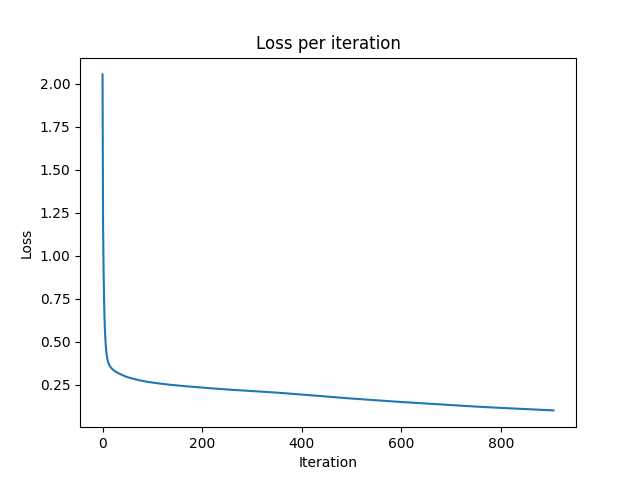
\includegraphics[width=0.75\textwidth]{best-train.png}
        \end{center}
              \begin{center}
            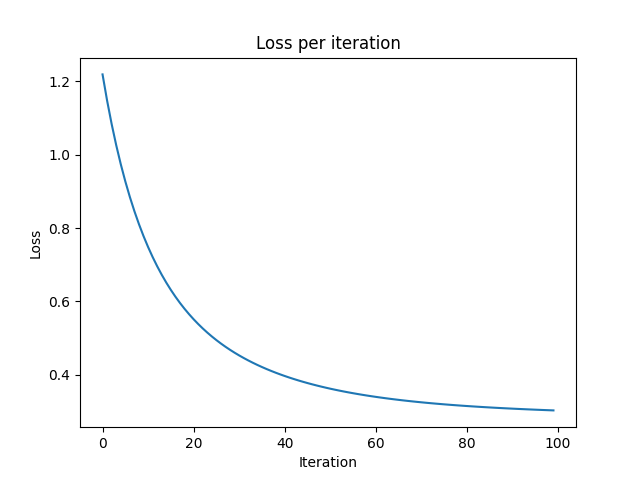
\includegraphics[width=0.75\textwidth]{best-test.png}
        \end{center}
              \begin{center}
            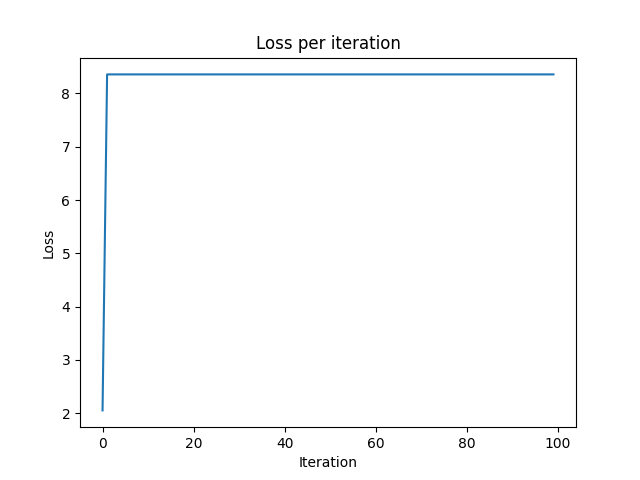
\includegraphics[width=0.75\textwidth]{worst-train-test.png}
        \end{center}
\begin{table}[!b]
    \centering
    \begin{tabular}{|l|l|l|l|l|l|}
    \hline
        Warstwy & Iteracje & Tempo uczenia & Loss & Dokładność tren. & Dokładność test. \\ \hline
        [13, 8, 1] & 10 & 0.001 & 0.40940036752387515 & 82 & 64 \\ \hline
        [13, 8, 1] & 100 & 0.001 & 0.2624329092132141 & 87 & 70 \\ \hline
        [13, 8, 1] & 500 & 0.001 & 0.16937331114162654 & 92 & 72 \\ \hline
        [13, 8, 1] & 1000 & 0.001 & 0.10021432493819211 & 98 & 72 \\ \hline
        [13, 1] & 100 & 0.001 & 0.3025827881814696 & 87 & 79 \\ \hline
        [13, 3, 1] & 100 & 0.001 & 0.42985408397547564 & 81 & 74 \\ \hline
        [13, 8, 1] & 100 & 0.001 & 0.2624329092132141 & 87 & 70 \\ \hline
        [13, 8, 8, 1] & 100 & 0.001 & 0.2174539200218492 & 88 & 72 \\ \hline
        [13, 8, 1] & 100 & 0.9999 & 8.357531178906184 & 54 & 59 \\ \hline
        [13, 8, 1] & 100 & 0.1 & 8.357531178906184 & 54 & 59 \\ \hline
        [13, 8, 1] & 100 & 0.01 & 0.1512313671335886 & 95 & 74 \\ \hline
        [13, 8, 1] & 100 & 0.001 & 0.2624329092132141 & 87 & 70 \\ \hline
        [13, 8, 1] & 100 & 0.0001 & 0.40063835340661175 & 81 & 62 \\ \hline
    \end{tabular}
    \caption{Wyniki trenowania sieci w zależności od warstw, liczby iteracji i tempa uczenia się dla zbioru treningowego i testowego}
\end{table}
       % \begin{center}
       %      \includegraphics[width=0.75\textwidth]{Linear_Scrap.png}
       %  \end{center}
\section{Porównanie z sklearn.neural\_network.MLPClassifier}

\section{Podsumowanie}

\noindent

\end{document}
